\documentclass[13pt, a4paper]{article}
\usepackage[english]{babel}
%\usepackage[utf8]{inputenc}
\usepackage{booktabs}
\usepackage{array}
\usepackage{mathptmx}[ptm]
\usepackage{a4wide,amssymb,epsfig,latexsym,hhline,fancyhdr}
\usepackage[normalem]{ulem}
\usepackage{tabularx}
\usepackage[makeroom]{cancel}
\usepackage{amsmath}
\usepackage{amsthm}
\usepackage{multicol,longtable,amscd}
\usepackage{diagbox}%Make diagonal lines in tables
\usepackage{alltt}
\usepackage[framemethod=tikz]{mdframed}% For highlighting paragraph backgrounds
\usepackage{caption,subcaption}
\usepackage{float}

\usepackage{lastpage}
\usepackage[lined,boxed,commentsnumbered]{algorithm2e}
\usepackage{enumerate}
\usepackage{enumitem}
\usepackage{color}
\usepackage{graphicx}							% Standard graphics package
\usepackage{multirow}
\usepackage{rotating}
\usepackage{graphics}
\usepackage{geometry}
\usepackage{setspace}
\usepackage{tikz}
\usepackage{listings}

\usepackage{fontspec}
\usepackage[hyphens]{url}

\setmainfont{Times New Roman}
\usepackage[unicode]{hyperref}

\hypersetup{colorlinks=true, linkcolor=blue, urlcolor=blue, citecolor=blue}
\geometry{a4paper, margin=2.5cm}
\lstset{
    basicstyle=\ttfamily\small,
    breaklines=true,
    columns=fullflexible,
    frame=single,
    backgroundcolor=\color{gray!5},
}

% Visual evidence is added after the corresponding implementation or demo is available.
\newcommand{\figureplaceholder}[2]{%
\begin{figure}[H]
    \centering
    \fbox{\parbox[c][#1][c]{0.86\textwidth}{\centering\itshape #2}}
    \caption{#2}
\end{figure}%
}

\title{Sales Pipeline Demo \\ \large Technical Report}
\author{Vũ Hoàng Tùng}
\date{\today}

\begin{document}
\maketitle
\tableofcontents
\newpage

% ============================================================
\section{Introduction}
% ============================================================
\subsection{Resources}
GitHub repo: \url{https://github.com/TUng1872004/Sale-app.git}\\
\subsection{Context}
Following the requirements, this is a business model under demo: \textbf{Sale} $\rightarrow$ \textbf{Agency (Đại lý)} $\rightarrow$
\textbf{Opportunity (Cơ hội bán hàng)}. A sales rep owns a set of agencies; each agency can carry
multiple open or closed sales opportunities that need tracking through a pipeline. The brief's functional requirements 
are intentionally high-level, leaving the author to decide domains, 
functionality, and implementation details. 
\\\\
It is actually a difficult task for me since I have no experience in sales. So in order to understand the domain, I decided to 
build a demo around this dataset, which is a real-world dataset of sales opportunities. {Dataset.} named 
CRM Sales Opportunities dataset (\url{https://mavenanalytics.io/data-playground/crm-sales-opportunities}), which ships four
CSVs already close to the target schema: 
\begin{itemize}
    \item Table accounts: represent account of customers
    \item Table products: Products that companies sold
    \item Table sales\_pipeline: shows exactly the spirit of the objectives: a standard sale tracking table tracking employee, customers, stage and revenue
    \item Table sales\_teams: team with members and their managers
\end{itemize}
Using real, messy third-party data (missing
account references, free-text loss reasons, etc.) forces the ETL and domain rules to handle
actual edge cases instead of clean synthetic fixtures. See \S\ref{subsec:etl} for how import
gaps were handled.
\subsection{Scope and constraints}
Given this is a 1 day demo and how unexperienced I am in sales, a lot of things I have here based on naive assumption 
of the data with a few usecases I can reasoning about. I do not try to anticipate all cases, rather this project aims to show that 
I can anticipated most cases and propose effective solutions, given more time or actual project planning. 
\\\\
For now the expected scopes are:
\begin{itemize}
    \item Complete minimal requirements: Sale $\rightarrow$ Agency $\rightarrow$ Opportunity, with domain rules and unit tests.
    \item Document the AI usage and engineering decisions.
    \item Document the assumptions and trade-offs, the limitations and open questions.
    \item System Architecture and design options that fit the requirements and business model as good as possible.
    \item Implement the recommendation engine as an AI feature, with benchmark. 
\end{itemize}

\subsection{How I will use AI}
The brief explicitly allows AI usage, but asks for it to be documented. I will use Claude to support my reasoning and implementation, 
with well defined requirements, planning and supervision from me.

The standard workflow of Claude that I use here as well as in all other projects is as follows:
\begin{enumerate}
    \item Write README.md with requirements and functional specifications. Do it by me
    \item Prompt to Claude for skeleton folder structure and module proposal. This will affect the architecture and design of the 
    project, so AI will init standard folders with direct adjustment from me.
    \item Modules then stacks. Step 2 creates a solid structure. AI will suggest stacks and implementation with my approval. Also
    testcases will be generated by AI, decoupled for each module.
    \item Craft plan and design for each module. I will prompt to Claude for a plan and design, code then generated after approval.
    \item Test and benchmark. I recheck testcases and benchmark generated in previous steps and test core features in each group by hand
    , then report the result.
\end{enumerate}
Current execution of steps are heavily focused on modularity for further maintenance and fixing, since:
\begin{itemize}
    \item It is supported by FastAPI well via libraries dedicated to Dependency Injection pattern
    \item Good for tests, error fix each models without affecting others.
    \item In that modular blueprint, AI rarely makes mistakes and all are revertable module by module easily with git reset.
\end{itemize}

% ============================================================
\section{Functional requirements}

This demo addresses the mandatory business chain \textbf{Sale $\rightarrow$ Agency $\rightarrow$
Opportunity}. The smallest complete flow is: create a Sale, create an Agency, assign its
owner, create an opportunity, and view an overview of the resulting pipeline. The system
prioritizes correct relationships, explicit validation, and explainable metrics over the
feature breadth of a production CRM.

\subsection{Roles and access boundaries}

Three roles define the reporting hierarchy: \texttt{SALER}, \texttt{MANAGER}, and
\texttt{DIRECTOR}. A Saler works only on their assigned opportunities; a Manager can view and
manage work within their team; a Director has global oversight. Minimum authorization rules
are implemented as domain functions, rather than relying on a UI to hide prohibited actions.

\subsection{Core functions}

\begin{itemize}
    \item Maintain Sales, including role, manager, active status, and ownership relationship.
    \item Maintain Agencies and record the Sale currently responsible for each Agency.
    \item Create, update, assign, and delete opportunities linked to exactly one Agency and one owner.
    \item Move opportunities through an explicit, validated sales pipeline.
    \item View open opportunities as a four-stage Kanban board scoped to the current team.
    \item Reassign an Agency while preserving ownership history and revenue attribution for
        closed opportunities.
    \item Calculate pipeline value, won revenue, win rate, stage distribution, loss reasons,
        stale opportunities, and workload.
    \item Recommend an assignment priority from measurable deal and historical-performance
        factors.
    \item Roll back data changes on failed validation or domain-rule rejection, so no partial updates leave the database in an inconsistent state.
\end{itemize}

\subsection{Role-specific requirements}

The dashboard explains recommendations directly from data and score factors; no Gemini or
other generated narrative is required.

\subsubsection{Director}

\textit{Management tab}
\begin{itemize}
    \item View the overall monthly revenue chart on entry.
    \item View \texttt{manager\_logs}, including team-revenue changes and manager reports;
        each log can open its full report document from shared MinIO storage for this demo.
    \item View best and worst teams for a selected month, ordered against the standard EMA.
    \item Drill into a team to view its revenue chart, Saler contribution, and progress.
    \item View that team's scoped Opportunity Kanban after opening its team page.
    \item Deactivate a Saler directly after recording a reason document. The destructive action
        uses a three-second hover-to-arm confirmation that turns red only when ready.
\end{itemize}

\textit{Business tab}
\begin{itemize}
    \item Create, view, update, and delete opportunities; select multiple opportunities and
        assign them to a team.
    \item Rank opportunity--Saler matches using overall win rate, field-specific Saler win
        rate, team win rate in that field, field revenue, and average time to win. Factors are
        normalized dynamically, then reranked by Position as the first-order criterion: a
        non-matching position is placed below matching positions.
\end{itemize}

\subsubsection{Manager}

\textit{Management tab}
\begin{itemize}
    \item View the team's monthly revenue chart, best and worst performers, and comparison
        with the standard EMA.
    \item View the team's open pipeline as a Kanban board on the dashboard.
    \item View searchable \texttt{salers\_logs}, including revenue changes, reports, and
        requests. Each record can open its full report document from shared MinIO storage.
    \item Propose, rather than execute, a Saler offboarding action. The same three-second
        hover-to-arm confirmation applies, and the request is sent to the Director.
    \item Create and review Frequent Reports about staff, sales details, business issues, or
        management issues.
\end{itemize}

\subsubsection{Saler}

\begin{itemize}
    \item Update sale details through a \texttt{Sale\_Report} with all required fields.
    \item View unhandled opportunities and submit a take-charge request to the Manager.
    \item Create and submit Frequent Reports about sales, business, or workplace issues.
    \item Set a seriousness level on Frequent Reports; the level controls the colour and text
        prominence shown in the superior's log table.
\end{itemize}



% ============================================================




% ============================================================
\section{System architecture and design choices}
% ============================================================

Figure\ref{fig:architecture} is the layered architecture used for this project. The green \textit{View}
block contains authentication, the Jinja2 UI, and FastAPI routes. The blue \textit{Controller}
boundary contains two modules: \textit{Service}, which executes workflows requested by the API,
and \textit{Domain}, which makes pure business decisions. The orange \textit{Data /
Infrastructure} block provides repositories over SQLModel/SQLite and a MinIO storage facade.

\begin{figure}[H]
    \centering
    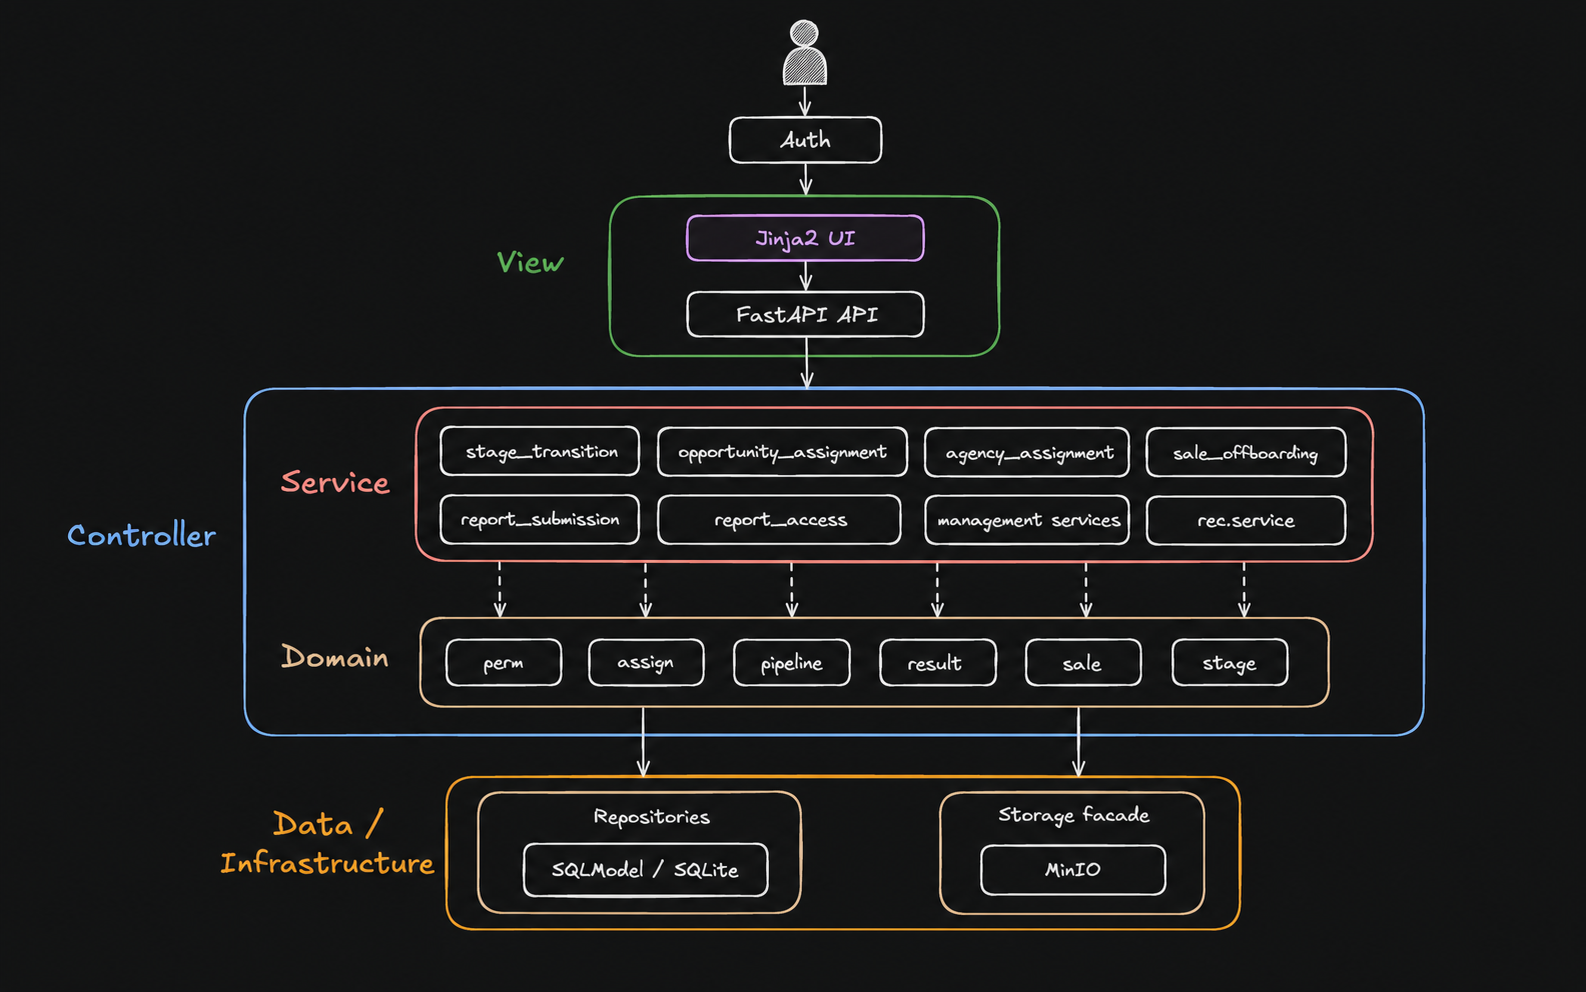
\includegraphics[width=1.00\textwidth]{img/arch.png}
    \caption{Module architecture. Solid arrows are direct dependencies (import); dashed arrows are dependency injection from Service to Domain.}
    \label{fig:architecture}
\end{figure}

\subsection{Design choice}
\subsubsection{Layered architecture}
As shown in Figure \ref{fig:architecture}, standard operational flow is \textit{controller $\rightarrow$ service $\rightarrow$ domain,
repository, and infrastructure}. A service may write through the SQLModel session and call the
storage facade, while the domain layer must not depend on HTTP, SQLModel sessions, MinIO, or
FastAPI. Read-only dashboard pages may call repositories directly because they do not execute
a business workflow, but cannot access domain. This decouples the layers, allowing:
\begin{itemize}
    \item Decouple of FE and BE development, so that FE can be developed in parallel with BE. All FE cares are API endpoints and data format, 
    which are defined in the controller layer. Since schema in core shared module, the core logic are in sync.
    \item Unit testing of domain rules without a running web server, database, or MinIO instance.
    \item High level abstraction: service orchestrates domain rules, not repo directly. Requests cannot bypass domain rules, 
    so the business logic is centralized and testable, repos are completely safe.
\end{itemize}

I utilize FastAPI to inject the current user, database session, and storage facade
into controller handlers; configuration injects settings into the database and storage
providers. Guarantees that the domain layer is pure and testable without a running web server, database, or MinIO instance.
Moreover, the secret information are not copied, only injected into the providers, so the domain layer is also secure. Later use 
of hashed password, access or refresh tokens and other sensitive information will be safe as well.
\subsubsection{Why visitor pattern}
Current data from Kaggle: unchanged data, no new data, no new features, no new requirements. Visit pattern decouple logic and data, 
so new algorithms and data structures can be easily extended by adding new visitors without 
changing the existing code, or adding any methods.

\subsection{Module and submodule mapping}

Table \ref{tab:diagram-modules} follows Figure \ref{fig:architecture}, with
\texttt{core/} added as a peer source module. The diagram groups the four management files
into one \textit{management services} box; the table expands that box to its source files.

\small
\begin{longtable}{@{}p{0.14\textwidth}p{0.20\textwidth}p{0.18\textwidth}p{0.22\textwidth}p{0.20\textwidth}@{}}
\caption{Architecture modules and submodules.}\label{tab:diagram-modules}\\
\toprule
\textbf{Module} & \textbf{Module purpose} & \textbf{Submodule} & \textbf{File path} & \textbf{Submodule purpose} \\
\midrule
\endfirsthead
\toprule
\textbf{Module} & \textbf{Module purpose} & \textbf{Submodule} & \textbf{File path} & \textbf{Submodule purpose} \\
\midrule
\endhead
\bottomrule
\endfoot

View & Handle user interaction. & Auth & \path{app/auth/deps.py} & User and role guards. \\
\midrule
View & Handle user interaction. & Jinja2 UI & \path{app/templates/*.html} & Rendered pages. \\
\midrule
View & Handle user interaction. & FastAPI API & \path{app/api/web.py} & Routes and responses. \\
\midrule
Controller / Service & Run API workflows. & stage\_transition & \path{app/services/stage_transition.py} & Change stage; write report and log. \\
\midrule
Controller / Service & Run API workflows. & opportunity\_assignment & \path{app/services/opportunity_assignment.py} & Assign individual/bulk deals and requests. \\
\midrule
Controller / Service & Run API workflows. & agency\_assignment & \path{app/services/agency_assignment.py} & Reassign Agencies and log history. \\
\midrule
Controller / Service & Run API workflows. & sale\_offboarding & \path{app/services/sale_offboarding.py} & Execute or decide offboarding. \\
\midrule
Controller / Service & Run API workflows. & report\_submission & \path{app/services/report_submission.py} & Store reports and logs. \\
\midrule
Controller / Service & Run API workflows. & report\_access & \path{app/services/report_access.py} & Authorize report links. \\
\midrule
Controller / Service & Run API workflows. & management services & \path{app/services/sale_management.py} & Manage Sales and Position. \\
\midrule
Controller / Service & Run API workflows. & management services & \path{app/services/agency_management.py} & Manage Agencies. \\
\midrule
Controller / Service & Run API workflows. & management services & \path{app/services/opportunity_management.py} & Create, update, and delete Opportunities. \\
\midrule
Controller / Service & Run API workflows. & management services & \path{app/services/overview.py} & Build scoped Kanban views. \\
\midrule
Controller / Service & Run API workflows. & rec.service & \path{app/rec/service.py} & Rank Saler candidates. \\
\midrule
Controller / Domain & Apply business rules. & perm & \path{app/domain/perm.py} & Check permissions. \\
\midrule
Controller / Domain & Apply business rules. & assign & \path{app/domain/assign.py} & Decide reassignment behaviour. \\
\midrule
Controller / Domain & Apply business rules. & pipeline & \path{app/domain/pipeline.py} & Stale-stage thresholds. \\
\midrule
Controller / Domain & Apply business rules. & result & \path{app/domain/result.py} & Typed rule outcomes. \\
\midrule
Controller / Domain & Apply business rules. & sale & \path{app/domain/sale.py} & Guard offboarding. \\
\midrule
Controller / Domain & Apply business rules. & stage & \path{app/domain/stage.py} & Guard stage changes. \\
\midrule
Core & Share application configuration and schema. & config & \path{app/core/config.py} & Application settings. \\
\midrule
Core & Share application configuration and schema. & labels & \path{app/core/schema/labels.py} & Display labels. \\
\midrule
Core & Share application configuration and schema. & models & \path{app/core/schema/models.py} & SQLModel tables and enums. \\
\midrule
Core & Share application configuration and schema. & report & \path{app/core/schema/report.py} & Report IDs, documents, and paths. \\
\midrule
Data / Infrastructure & Persist data and files. & Repositories & \path{app/repo/*.py} & Scoped database reads. \\
\midrule
Data / Infrastructure & Persist data and files. & SQLModel / SQLite & \path{app/db.py} & Engine and sessions. \\
\midrule
Data / Infrastructure & Persist data and files. & Storage facade & \path{app/storage.py} & Storage abstraction. \\
\midrule
Data / Infrastructure & Persist data and files. & MinIO & Docker Compose service & Report documents. \\
\end{longtable}
\normalsize
The table concludes the architecture and design choices, laying solid foundation to later implementation. 
The next section describes the domain rules that enforce the business logic.
% ============================================================
\section{Data model}
% ============================================================

Six tables implement the Sale $\rightarrow$ Agency $\rightarrow$ Opportunity chain, assignment
history, and separate manager/Saler audit logs. Defined in \texttt{app/core/schema/models.py} as SQLModel classes (single source of
truth for both the Python types and the SQL schema, migrated via Alembic).
\begin{figure}[H]
    \centering
    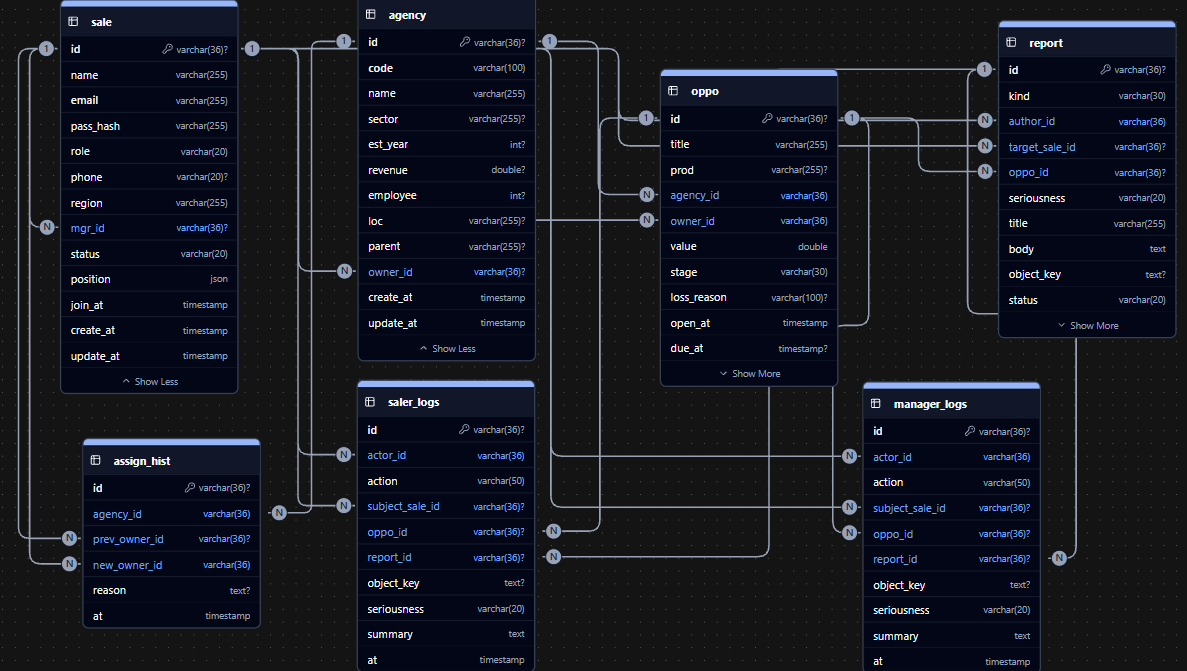
\includegraphics[width=1.00\textwidth]{img/db.png}
    \caption{Database schema.}
    \label{fig:db-schema}
\end{figure}

\subsection{Core entities}

\begin{description}
    \item[\texttt{Sale}] A user: Saler, Manager, or Director (\texttt{role} enum). Self-referential
        \texttt{mgr\_id} builds the reporting tree (\texttt{null} for Director). Carries
        \texttt{status} (ACTIVE/INACTIVE) rather than deleting the row on offboarding — see
        \S\ref{sec:assumptions}.
    \item[\texttt{Agency}] An account/customer. \texttt{owner\_id} points at the responsible
        Sale (nullable: an agency can be temporarily unowned, e.g. between reassignments).
    \item[\texttt{Oppo}] An opportunity tied to exactly one \texttt{Agency} and one owning
        \texttt{Sale}. Carries \texttt{stage}, optional \texttt{loss\_reason}, and timestamps
        (\texttt{open\_at}, \texttt{due\_at}, \texttt{close\_at}) that drive the staleness and
        scoring logic in \S\ref{sec:rec}.
    \item[\texttt{AssignHist}] Audit trail of ownership changes on an agency: previous owner,
        new owner, free-text reason, timestamp. Exists so "who owned this and why did it move"
        is answerable without inferring it from side effects.
\end{description}

\subsection{Relationships and integrity}

\begin{itemize}
    \item \texttt{Sale.mgr\_id} $\to$ \texttt{Sale.id} (self-FK, nullable) — reporting line.
    \item \texttt{Agency.owner\_id} $\to$ \texttt{Sale.id} (nullable) — current owner.
    \item \texttt{Oppo.agency\_id} $\to$ \texttt{Agency.id} (required) — every opportunity
        belongs to exactly one agency.
    \item \texttt{Oppo.owner\_id} $\to$ \texttt{Sale.id} (required) — every opportunity has an
        explicit owner, independent of the agency's current owner (see \S\ref{sec:assumptions}
        on reassignment semantics).
    \item A composite index on \texttt{(stage, open\_at)} backs the stale-opportunity query
        (filter to open stages, then compare age) — added after the query pattern was known,
        not speculatively.
\end{itemize}

% ============================================================
\subsection{ETL and data import}
\label{subsec:etl}
% ============================================================

\texttt{app/seed.py} imports the four Maven Analytics CSVs into the schema above. The import
is idempotent (safe to re-run) and skips rows that cannot map cleanly onto the schema:

\begin{itemize}
    \item 1{,}425 of ~8{,}800 source \texttt{sales\_pipeline} rows had a blank \texttt{account}
        field and were skipped — verified by direct inspection of the raw CSV that every
        skipped row is an open-stage deal, so closed-deal counts (4{,}238 Won / 2{,}473 Lost)
        are unaffected by the skip.
    \item Expected seed counts were corrected mid-implementation once the real 16\% skip rate
        was discovered, rather than leaving a stale target a future test run would fail
        against for a non-bug reason.
\end{itemize}

% ============================================================
\section{Domain rules}
\label{sec:domain-rules}
% ============================================================

Business logic lives in \texttt{app/domain/} as pure functions with zero I/O — no ORM
session, no HTTP, so every branch is directly unit-testable and independent of the framework
underneath it. Each function returns a \texttt{Result} (Ok/Err) rather than raising, so
callers get a typed reason code instead of parsing an exception message.
\begin{figure}[H]
    \centering
    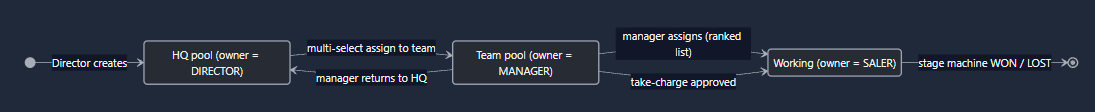
\includegraphics[width=1.00\textwidth]{img/oppo_cycle.png}
    \caption{Opportunity ownership lifecycle: From Director to Manager to Salers.}
    \label{fig:oppo-cycle}
\end{figure}


\subsection{Opportunity stage machine (\texttt{stage.py})}
\label{sec:stage-machine}

Normal sales states are \texttt{NEW $\to$ QUALIFY $\to$ PROPOSE $\to$ NEGOTIATE $\to$
\{WON, LOST\}}. \texttt{CLOSED} is an additional terminal state used only when a Director
deletes an open Opportunity that already has audit history. Rules enforced by
\texttt{can\_transition}:

\begin{itemize}
    \item Forward-only — a deal cannot move backward in the pipeline or skip a stage; both are
        rejected with distinct error codes (\texttt{BACKWARD}, \texttt{SKIP\_STAGE}).
    \item \texttt{WON}, \texttt{LOST}, and \texttt{CLOSED} are terminal — no further transition
        once closed (\texttt{TERMINAL}).
    \item Marking \texttt{LOST} requires a \texttt{loss\_reason}; marking \texttt{WON} rejects
        one being present. This trades a small amount of flexibility for data that is always
        explainable when a deal is lost.
\end{itemize}
\begin{figure}[H]
    \centering
    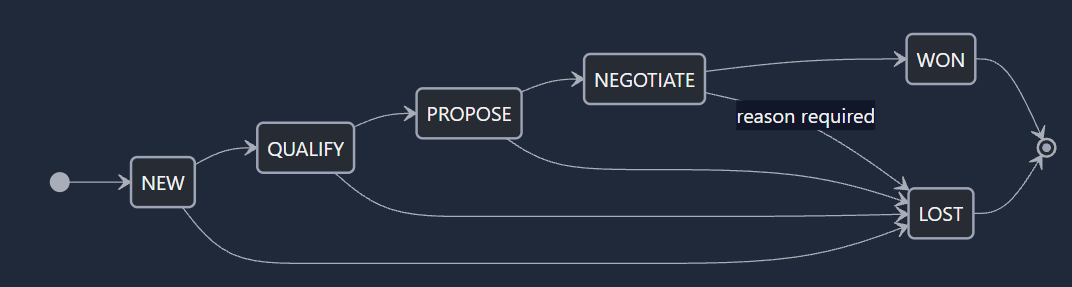
\includegraphics[width=1.00\textwidth]{img/stage.png}
    \caption{Opportunity stage transitions.}
    \label{fig:stage}
\end{figure}

\subsection{Reassignment (\texttt{assign.py})}

An agency's owner can change (\texttt{can\_reassign}) only to an \texttt{ACTIVE} Sale.
Reassigning an agency does \emph{not} blanket-move every historical opportunity: closed
opportunities (WON/LOST) stay credited to the original owner for revenue-attribution
integrity; open opportunities move with the agency to the new owner
(\texttt{oppo\_follows\_reassign}). This distinction was a deliberate answer to one of the
brief's open questions (\S\ref{sec:assumptions}).

\subsection{Permissions (\texttt{perm.py})}

One function per capability, checked in application code before any mutation — not left to
implicit role checks scattered across routes:

\begin{center}
\begin{tabular}{@{}ll@{}}
\toprule
Capability & Rule \\
\midrule
View an opportunity & Owner, owner's manager, or any Director \\
Reassign within a team & Manager of the agency's current owner, or Director \\
Reassign across teams & Director only \\
Deactivate a Sale & That Sale's manager, or Director \\
Export global data & Director only \\
\bottomrule
\end{tabular}
\end{center}

\begin{figure}[H]
    \centering
    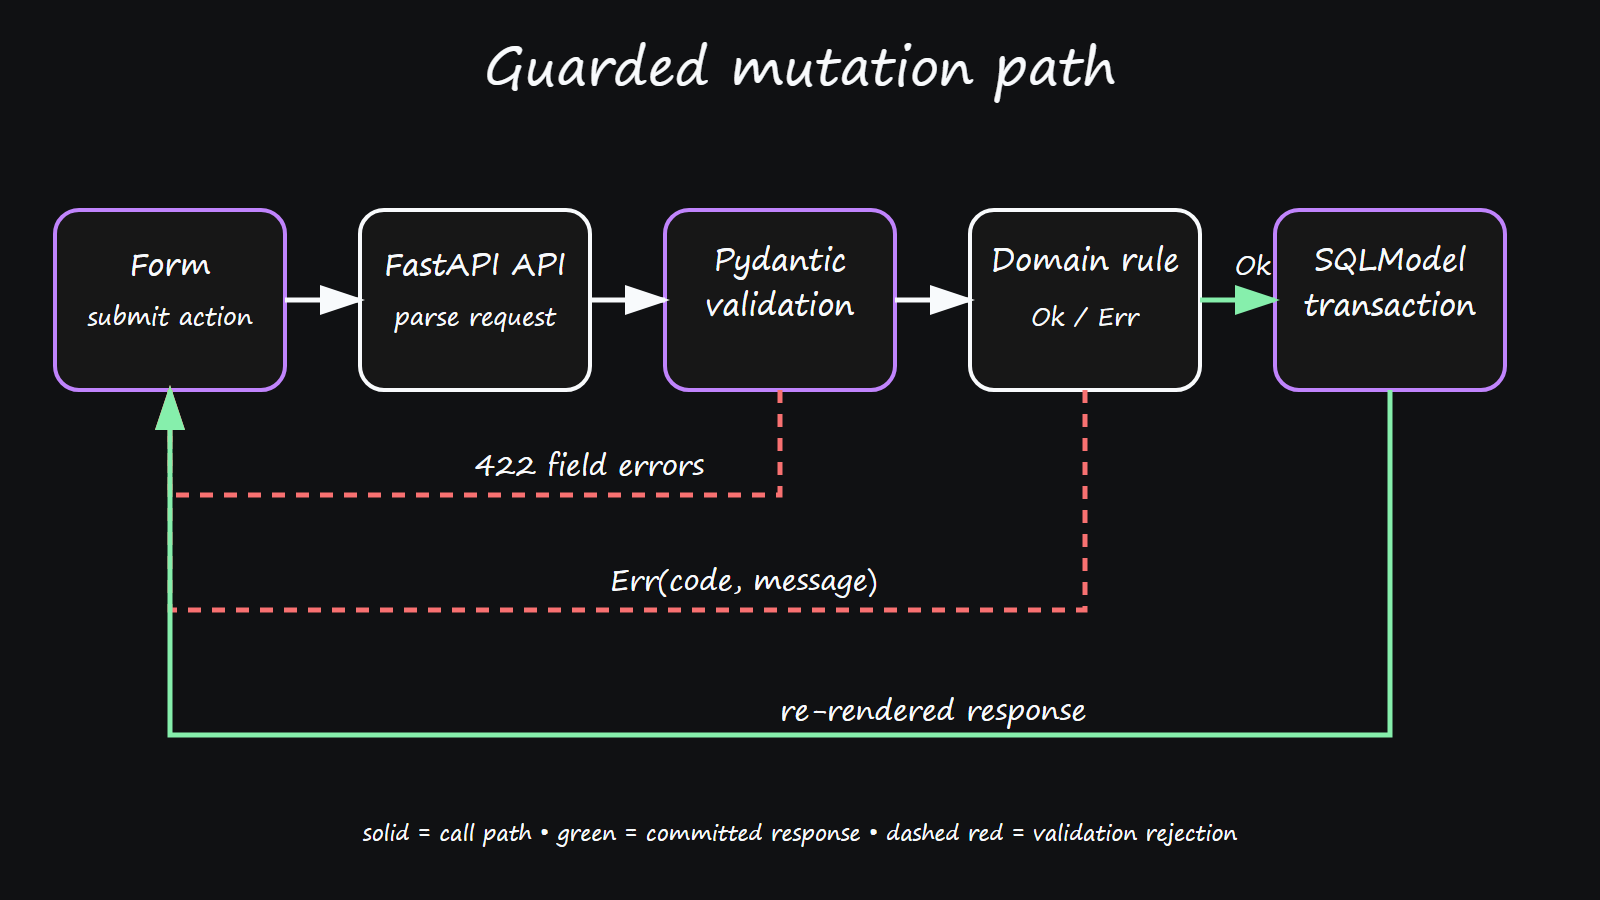
\includegraphics[width=\textwidth]{img/mutation_path.png}
    \caption{Guarded mutation path: validation and domain failures return without writing data; an accepted action commits in a transaction.}
    \label{fig:mutation-path}
\end{figure}

% ============================================================
\section{Recommendation / scoring engine}
\label{sec:rec}
% ============================================================

The Director-facing "recommend opportunities to salers" feature (per \texttt{README.md}'s
functional requirements) is implemented as a small scoring pipeline under
\texttt{app/rec/}, structurally a functional Visitor: each factor is an independent
function over a shared \texttt{DealCtx}, and \texttt{registry.py} folds their outputs into one
priority score — extending the model means adding one file to the \texttt{VISITORS} list, not
editing a growing branch tree.

\textbf{Factors (\texttt{rec/visitors/}):} stage weight, staleness (days in stage past a
per-stage threshold, capped impact), deal value vs. agency mean (outlier penalty), saler's
current load, and historical win-rate in that field/team. Weights and caps are centralized as
frozen constants in \texttt{rec/weight.py} rather than scattered literals, so tuning is a
one-file change.

\subsection{Visitor pattern for recommendation engine}

The opportunity-priority scorer applies a \emph{functional Visitor} pattern. Instead of a
classic object-oriented double-dispatch design, \texttt{DealCtx} is the element being visited
and each function in \texttt{app/rec/visitors/} implements the same callable protocol:
\texttt{DealCtx $\rightarrow$ Factor | None}. The functions are registered in the ordered
\texttt{VISITORS} list in \texttt{registry.py}; the registry invokes every visitor, keeps the
non-empty factors, and sums their impacts into a \texttt{Score}.

This design keeps visitors pure: the caller prepares a complete \texttt{DealCtx}, so visitor
functions perform no database or network I/O. Adding a scoring factor therefore means adding
one visitor file and registering it, without changing the existing factor implementations.
The resulting \texttt{Factor} objects retain a signal name and Vietnamese display explanation,
so a recommendation can be explained from its component scores rather than from generated
narrative.

The candidate-Saler recommender in \texttt{rec/service.py} is a separate workflow. Its learned
model is a binomial Generalized Linear Model (GLM), not ordinary linear regression: the model
uses standardized overall win rate, field-specific win rate, team field win rate, field revenue,
and average days to win. The benchmark artifact stores the scaler, GLM coefficients, and its
selection result; runtime retains a deterministic fallback if that artifact is invalid. Both
mechanisms remain explainable, but the functional Visitor pattern specifically describes the
opportunity-priority pipeline in \texttt{rec/registry.py}.

\begin{figure}[H]
    \centering
    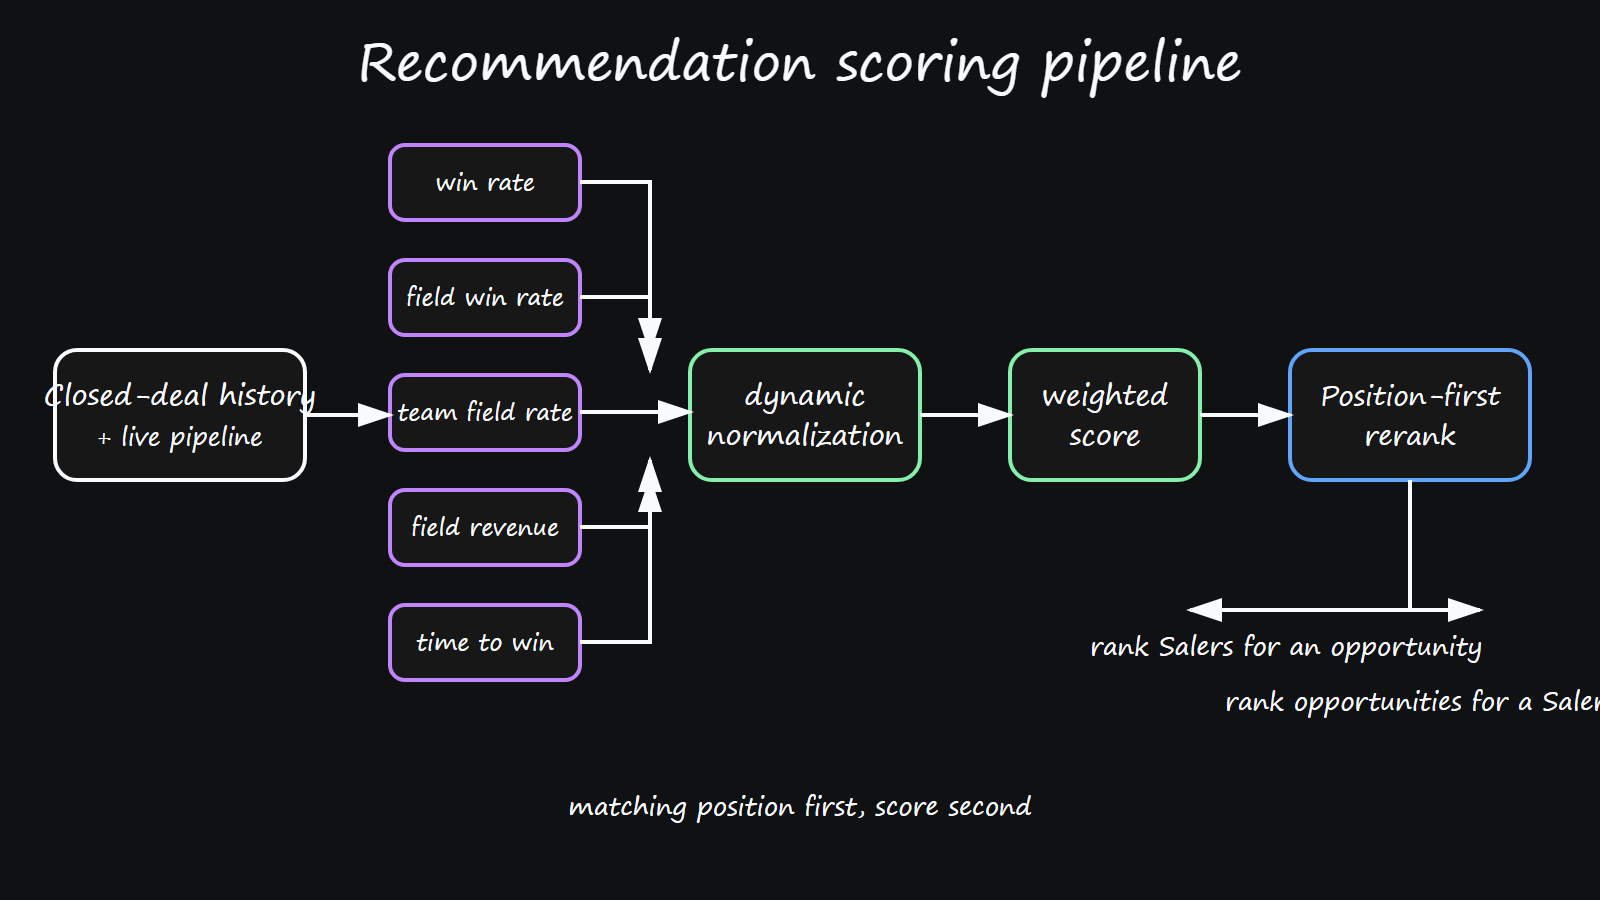
\includegraphics[width=\textwidth]{img/recommendation_pipeline.png}
    \caption{Recommendation scoring pipeline with dynamic normalization and Position-first reranking.}
    \label{fig:recommendation-pipeline}
\end{figure}

% ============================================================
\section{Testing}
% ============================================================

The suite contains 43 representative \texttt{pytest} cases, all passing at the time of
writing. It selects the decision boundaries and end-to-end flows that demonstrate each
delivery phase, rather than repeating every equivalent input permutation. The parameterised
Lost-stage test accounts for four of the 43 cases.

\small
\begin{longtable}{@{}p{0.12\textwidth}p{0.18\textwidth}p{0.55\textwidth}p{0.07\textwidth}@{}}
\caption{Representative automated tests by implementation phase.}\label{tab:test-phases}\\
\hline
\textbf{Phase} & \textbf{Test file} & \textbf{What is tested} & \textbf{Cases} \\
\hline
\endfirsthead
\hline
\textbf{Phase} & \textbf{Test file} & \textbf{What is tested} & \textbf{Cases} \\
\hline
\endhead
Phase 1: domain and access & \texttt{test\_stage.py} & \texttt{test\_negotiate\_to\_won\_allowed}, no skipped or backward stage, four open-stage-to-Lost paths, terminal Won/CLOSED, and required loss reason. & 10 \\
\hline
Phase 1: domain and access & \texttt{test\_assign.py} & Active/inactive reassignment target; open opportunity follows a reassignment while Won and Lost opportunities do not. & 4 \\
\hline
Phase 1: domain and access & \texttt{test\_sale.py} & Offboarding is rejected for a Sale owning agencies, an inactive Sale, or a Sale owning an open opportunity. & 3 \\
\hline
Phase 1: domain and access & \texttt{test\_perm.py} & Saler self/other scope, Manager own/other-team scope and team reassignment, plus Director cross-team reassignment. & 6 \\
\hline
Phase 2: data and ETL & \texttt{test\_repo.py} & Scoped list pagination, team membership, KPIs, stage and loss summaries, workload order, completed-month revenue, EMA, rankings, and stale boundary. & 3 \\
\hline
Phase 2: data and ETL & \texttt{test\_seed.py} & Deterministic agency-owner tie-break; initial seed, idempotent verification, reseed, and required Saler Position data. & 2 \\
\hline
Phase 2: dashboard & \texttt{test\_http.py} & Manager dashboard shows four scoped open-stage Kanban columns; Director team drill-down shows the selected team while excluding other teams. & 1 \\
\hline
Phase 3: workflows and HTTP & \shortstack{\texttt{test\_storage}\\\texttt{\_workflow.py}} & Upload/transaction compensation: SQL failure removes the uploaded document; upload failure makes no SQL write. & 2 \\
\hline
Phase 3: workflows and HTTP & \texttt{test\_http.py} & Login redirect and scope denial; Director CRUD, bulk assignment, history-protecting deletion, and offboarding guard; stage report and log; team-pool request/approval; dismissal reason and manager report storage. & 7 \\
\hline
Phase 4: recommendation & \texttt{test\_benchmark.py} & Exact Recall/Precision@3 and @5 calculation; Position match ranks ahead of a higher-scoring non-match. & 2 \\
\hline
Phase 4: recommendation & \texttt{test\_registry.py} & Won/Lost opportunities receive zero priority; open opportunities rank in descending priority. & 2 \\
\hline
Phase 4: recommendation & \shortstack{\texttt{test\_rec}\\\texttt{\_service.py}} & Invalid or incompatible benchmark artifact falls back to the deterministic recommender. & 1 \\
\hline
\textbf{Total} & & & \textbf{43} \\
\hline
\end{longtable}
\normalsize

The passing run provides repeatable verification evidence for the listed flows. \texttt{mypy}
runs clean across \texttt{app/} and \texttt{tests/} with a single documented, justified
suppression on a test helper's flexible kwargs (not production code).

\section{Conclusions and lessons learned}
% ============================================================
\subsection{Assumptions}
\label{sec:assumptions}
% ============================================================

The brief explicitly asks these to be asked and documented. The following are best-effort guesses based on the data, the business 
domain, and the requirements. They are not guaranteed to be correct, but they are consistent with the:

\begin{description}[leftmargin=0.4cm, style=nextline]
    \item[Sale nghỉ việc (offboarding) — how is old data handled?]
        A Sale is marked \texttt{INACTIVE}, never deleted. Historical opportunities and
        agencies keep their original \texttt{owner\_id} for reporting integrity; new work
        cannot be assigned to an inactive Sale (\texttt{can\_reassign} rejects it). Limitation:
        no automated "bulk reassign all of this Sale's open work" flow exists yet — a manager
        or director must reassign agencies individually.
    \item[Can an agency be transferred to another Sale?]
        Yes, within a manager's own team by that manager, or across teams by a Director only
        (\S\ref{sec:domain-rules}). Closed opportunities stay with their original owner; open
        ones move with the agency (\texttt{assign.py}). Trade-off: this optimizes for correct revenue attribution
        over a simpler "everything moves" rule.
    \item[What states can an opportunity be in, and how does it transition?]
        Six stages, forward-only, two terminal states, loss reason mandatory on loss —
        detailed in \S\ref{sec:stage-machine}.
    \item[Are duplicates allowed? Can created data be deleted?]
        Not yet enforced at the domain layer; the demo currently trusts the seed ETL's
        dedup logic (agency \texttt{code} is a unique slug of the account name) and does not
        expose hard deletes through the web layer — soft-deactivation
        (\texttt{status}) is the only lifecycle-ending operation modeled, deliberately, so
        history is never destroyed by a UI action.
    \item[Who can view or change data?]
        Three-role hierarchy (Saler / Manager / Director), enforced by the permission
        functions in \S\ref{sec:rec}'s domain-rules section, not by decorative role flags.
    \item[How are overview metrics computed?]
        Dashboard aggregates (pipeline value, won revenue, win rate, stage distribution, loss
        reasons, stale-opportunity count, per-saler workload) are computed in
        \texttt{app/repo/stats.py} directly from \texttt{Oppo} rows scoped by owner IDs,
        so the same formulas serve saler, manager, and director views without duplication.
        Exposed through the dashboard views described in \S\ref{sec:status}.
\end{description}

% ============================================================
\subsection{Achievement and current status vs the requirements}
\label{sec:status}
% ============================================================

\begin{center}
\begin{tabular}{@{}ll@{}}
\toprule
Layer & Status \\
\midrule
Schema \& migrations (Alembic) & Done \\
Seed / ETL from source CSVs & Done, idempotent \\
Domain rules (stage, assign, perm) & Done, unit-tested \\
Repository / query layer & Done, unit-tested \\
Recommendation / scoring engine & Done, unit-tested \\
HTTP routes (\texttt{app/api/}) & Done \\
Auth (\texttt{app/auth/}) & Done \\
Templates / UI (\texttt{app/templates/}) & Done \\
Opportunity CRUD and bulk assignment & Done, HTTP-tested \\
Scoped Manager/team Kanban & Done, HTTP-tested \\
\bottomrule
\end{tabular}
\end{center}

\begin{figure}[H]
    \centering
    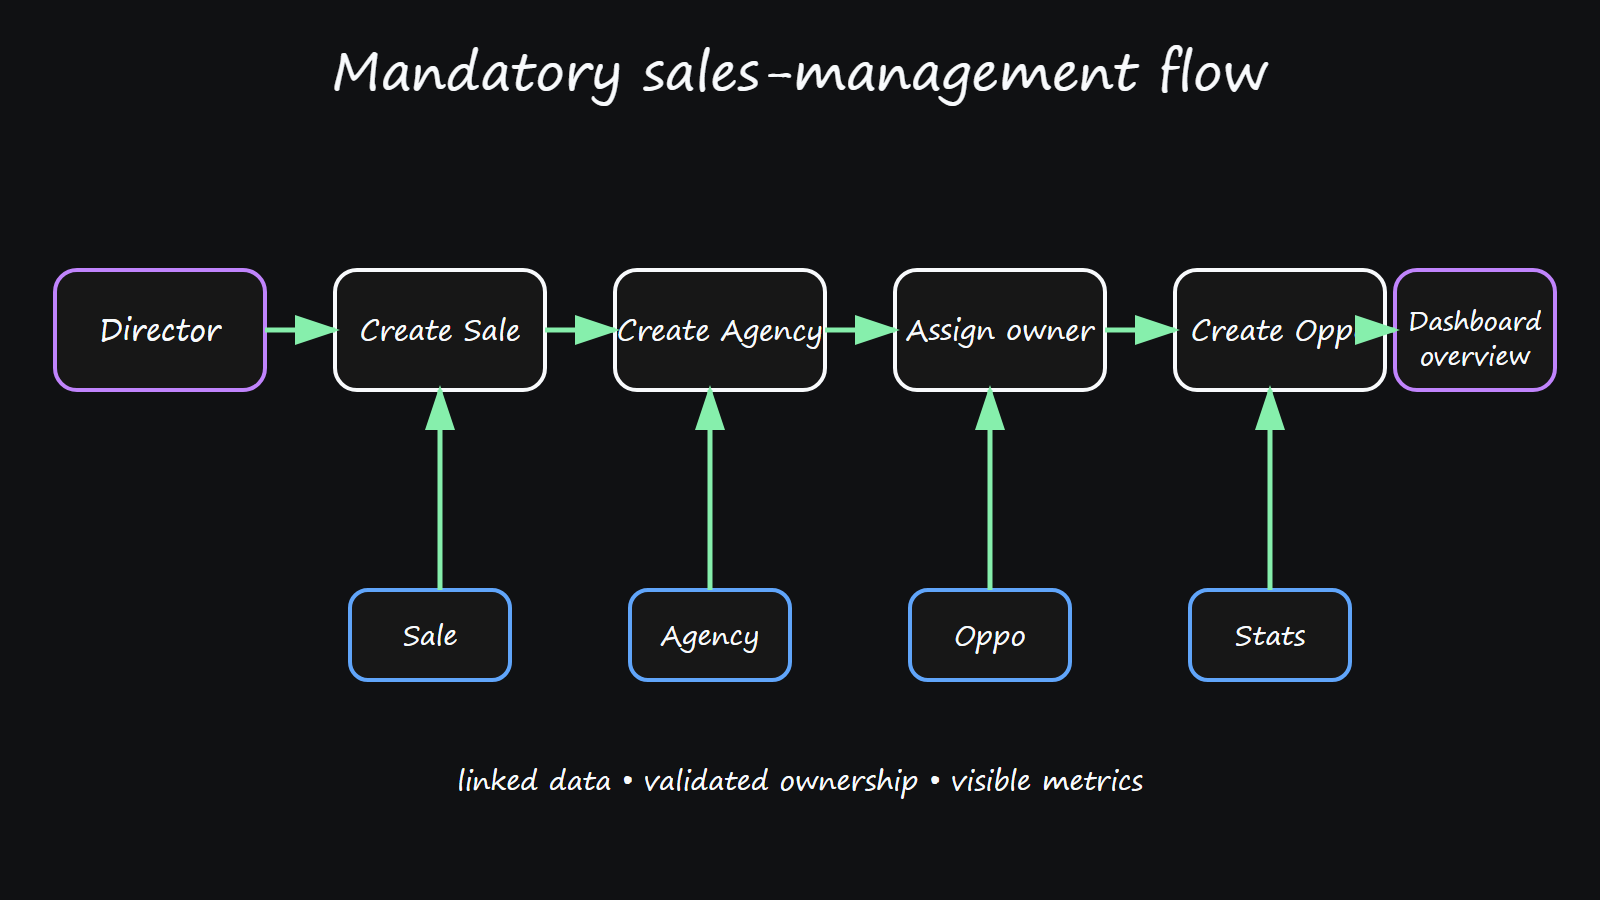
\includegraphics[width=\textwidth]{img/mandatory_flow.png}
    \caption{Mandatory Sales $\rightarrow$ Agency $\rightarrow$ Opportunity flow and the data it creates.}
    \label{fig:mandatory-flow}
\end{figure}

\begin{figure}[H]
    \centering
    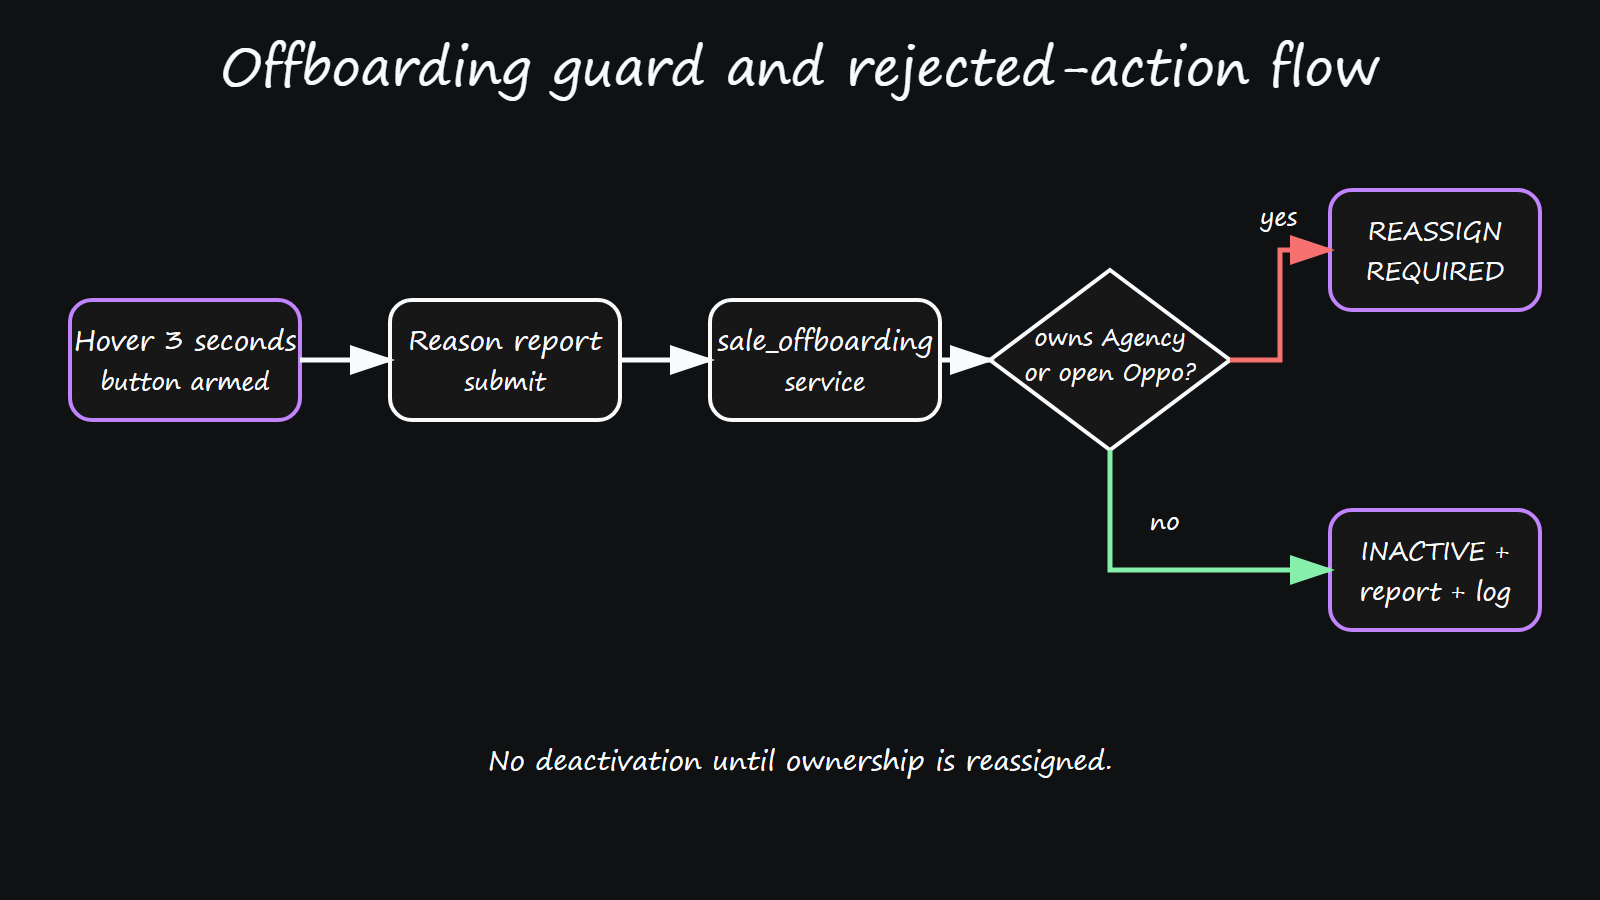
\includegraphics[width=\textwidth]{img/offboarding_guard.png}
    \caption{Rejected offboarding flow: ownership must be reassigned before a Sale can become inactive.}
    \label{fig:offboarding-guard}
\end{figure}

The full \textit{Create Sale $\rightarrow$ Create Agency $\rightarrow$ Assign $\rightarrow$
Create opportunity $\rightarrow$ View overview} flow is implemented end-to-end through the
server-rendered FastAPI interface. Routes receive the current user, database session, and
storage facade through dependency injection; write routes delegate to application services,
while read views use the shared repositories and dashboard statistics.

The Manager dashboard also presents the team's open pipeline as four Kanban columns:
\texttt{NEW}, \texttt{QUALIFY}, \texttt{PROPOSE}, and \texttt{NEGOTIATE}. Each card shows the
Opportunity, responsible Saler, value, and due date. A Director reaches the same scoped view by
opening \path{/teams/{manager_id}}; the service receives only that team's owner IDs, preventing
cards from another team from entering the board.

\begin{figure}[H]
    \centering
    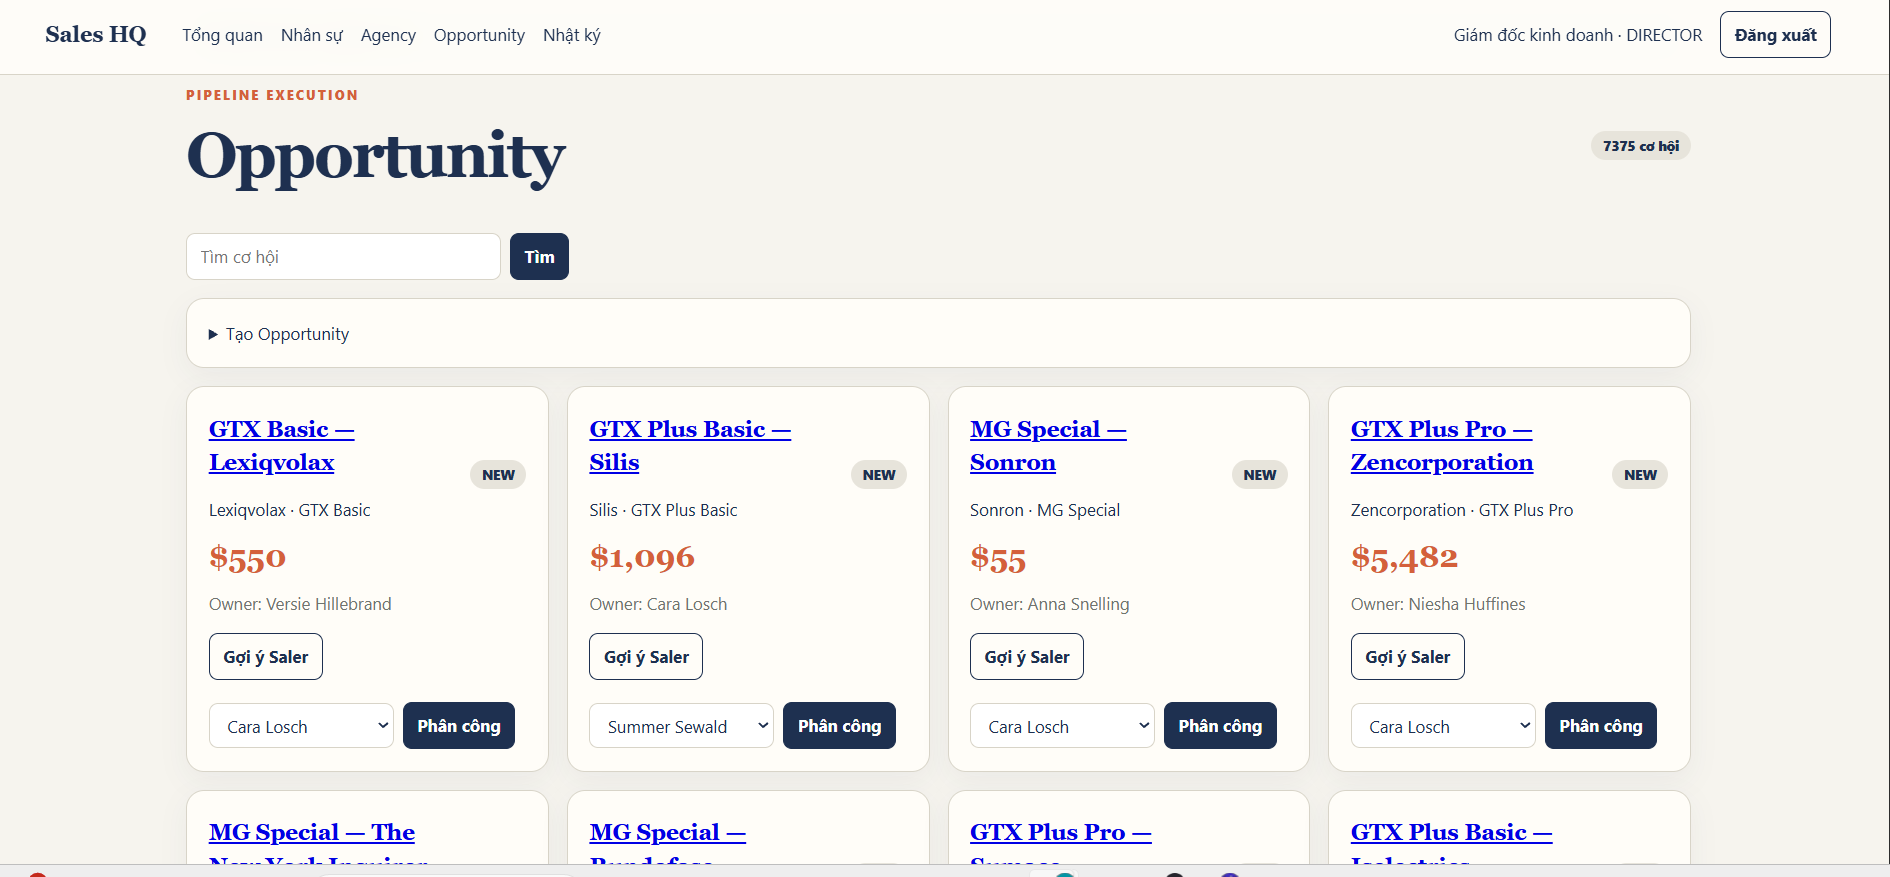
\includegraphics[width=\textwidth]{img/dic_overview.png}
    \caption{Director Opportunity Overview.}
    \label{fig:dic-overview}
\end{figure}

\begin{figure}[H]
    \centering
    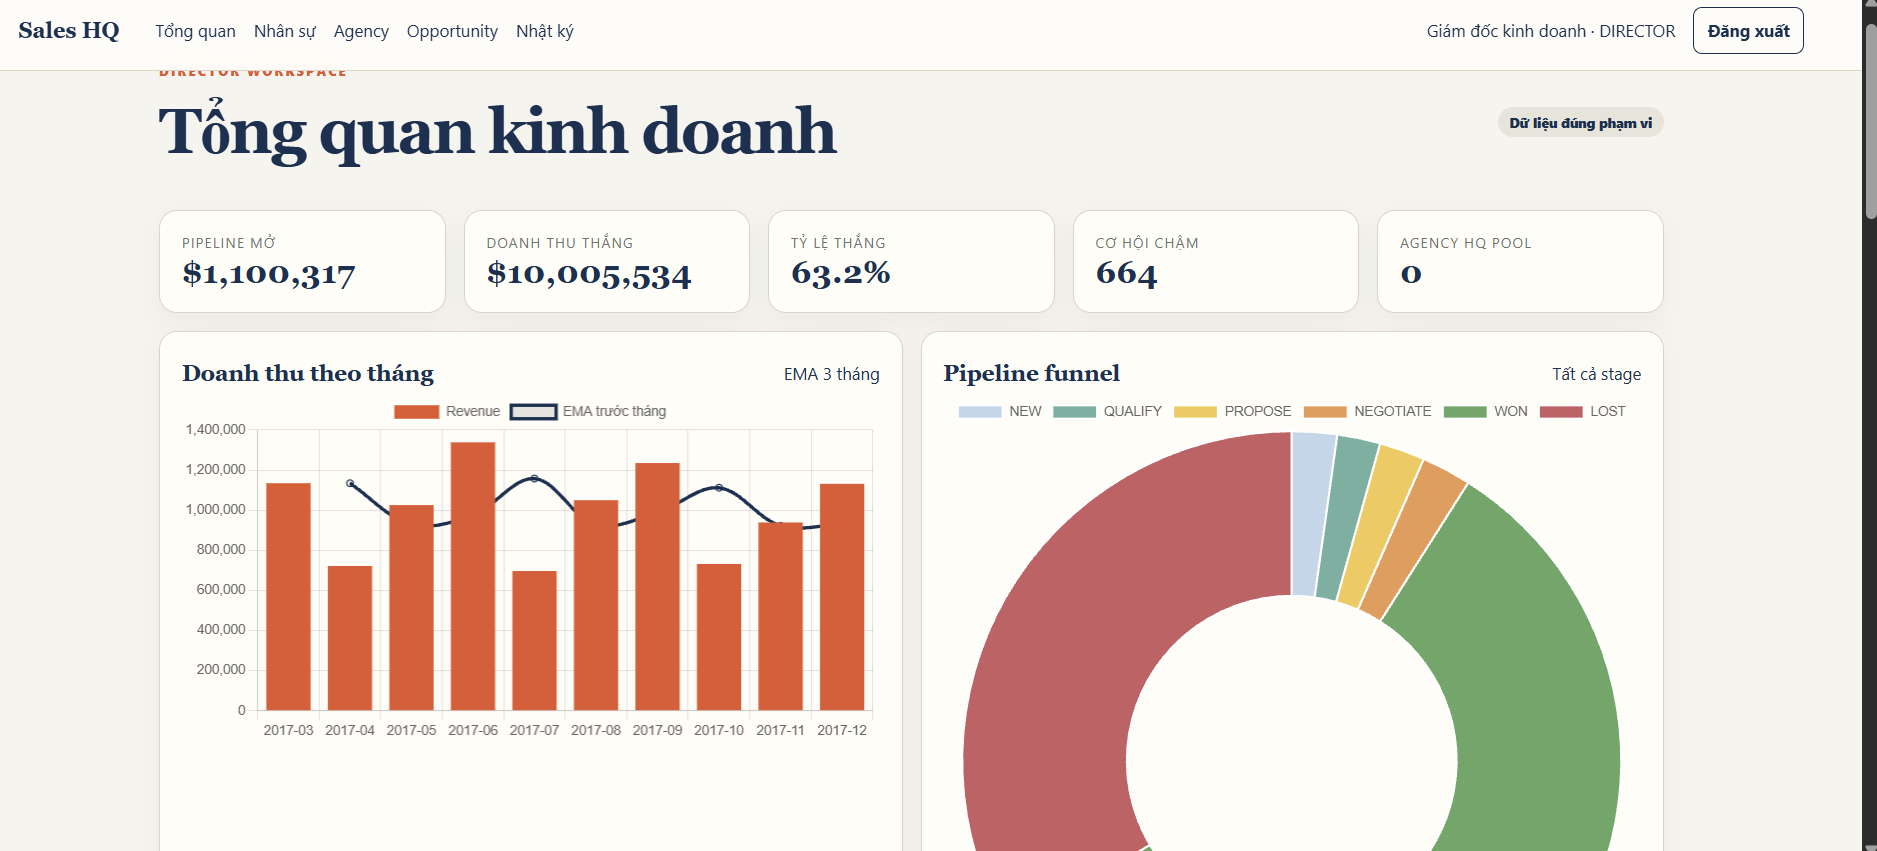
\includegraphics[width=\textwidth]{img/dict_chart.png}
    \caption{Director Revenue Chart.}
    \label{fig:dict-chart}
\end{figure}


\begin{figure}[H]
    \centering
    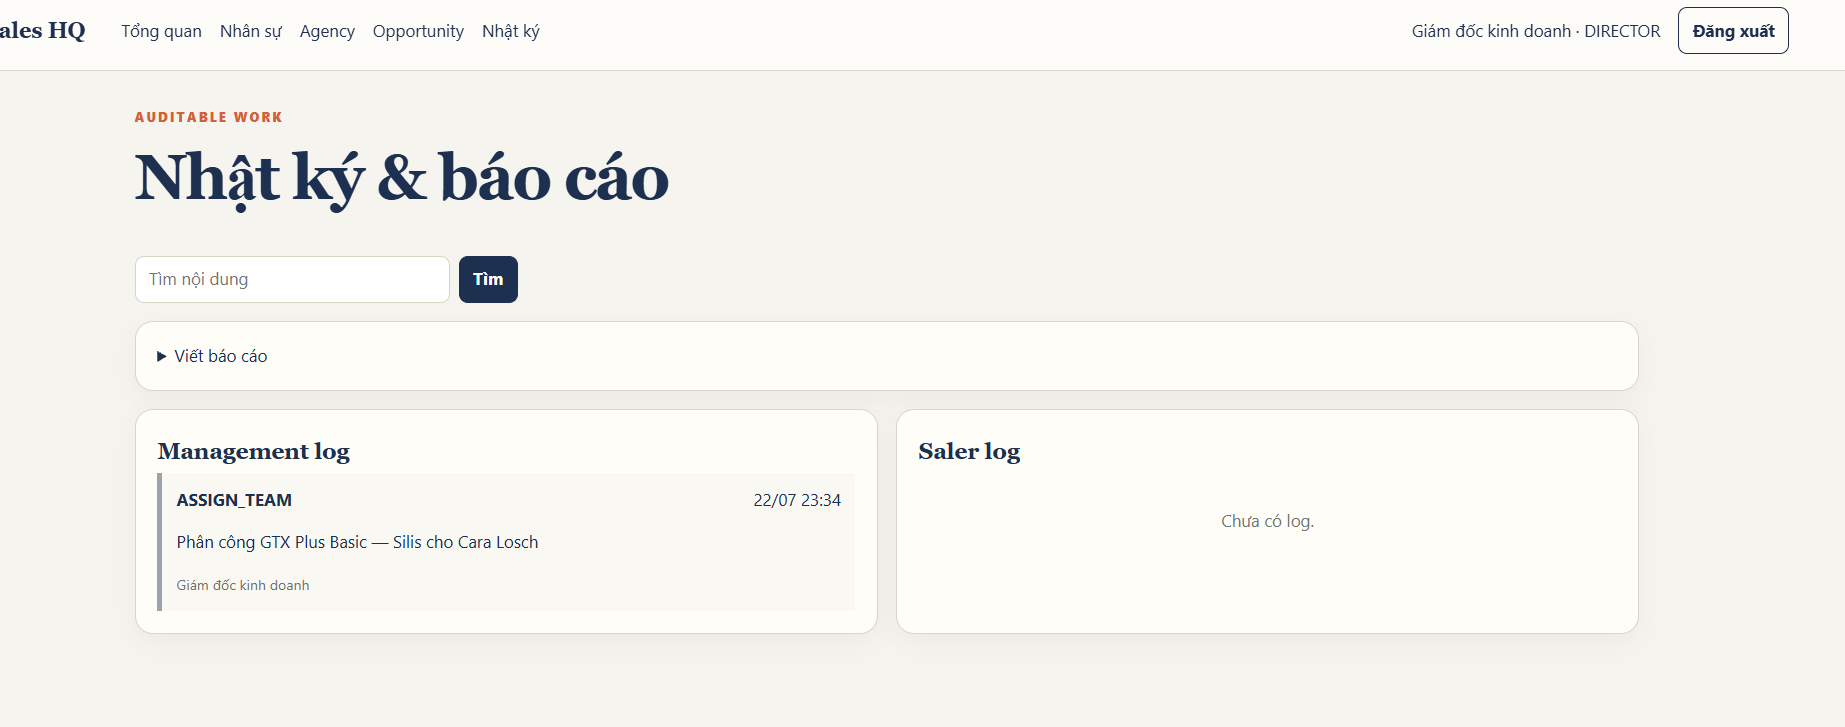
\includegraphics[width=\textwidth]{img/dict_log.png}
    \caption{Director Revenue Log.}
    \label{fig:dict-log}
\end{figure}

\begin{figure}[H]
    \centering
    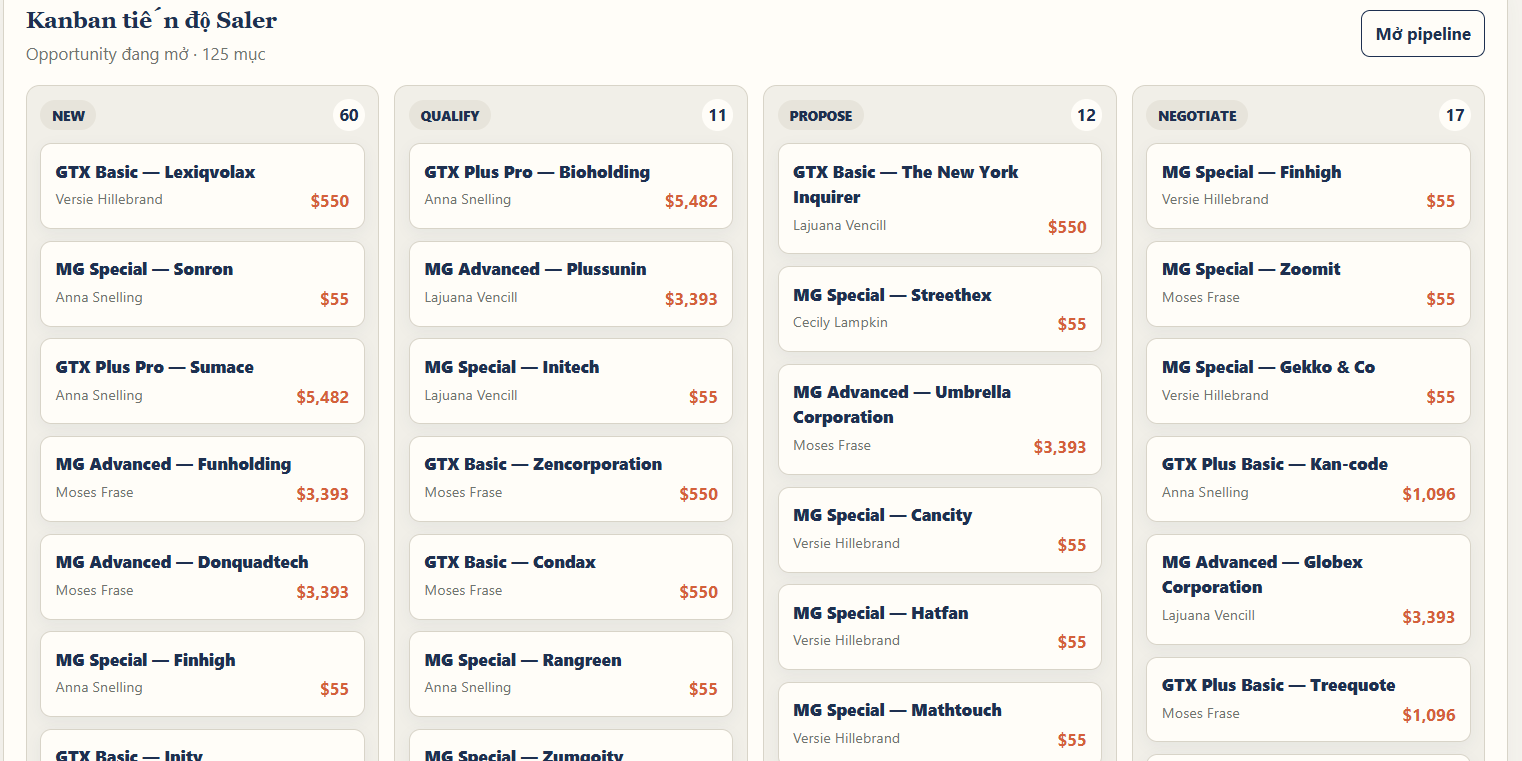
\includegraphics[width=\textwidth]{img/work_progress.png}
    \caption{Progress of Sales displayed in Kanban view.}
    \label{fig:work-progress}
\end{figure}
% ============================================================
\subsection{Limitations and future work}
% ============================================================
The following are the main points that need to be improved in the future:
\begin{itemize}
    \item No full browser end-to-end records yet, only technical documentation.
    \item No profile names are just meaningless string, cannot be clicked.
    \item No duplicate-detection semantics at the domain layer. A Director can hard-delete an
        open Opportunity without audit history; once history exists, deletion marks it
        \texttt{CLOSED} instead, preserving evidence.
    \item No automated bulk-reassignment on Sale offboarding.
    \item Domain modeling reflects best-effort assumptions from an data and business
        domain (sales operations), not exhaustive real-world coverage — by design, per
        \S\ref{sec:assumptions}. Need more time to research and understand the domain, 
        then adjust the model and rules accordingly.
    \item No production-grade security, hardening, logging, or monitoring. All is in a demo state, 
    with the exception of the domain rules and permission checks which is about logic more than real infrastructure.
    \item The binomial GLM is trained from historical CSV outcomes only. More live outcomes,
        richer business features, and periodic retraining are needed before treating its ranking
        as production-quality prediction.
    \item AI can be used for autonomous sales management, but it is not implemented yet, since data with such short field body 
    make GenAI a trivial task. If there are more complex case with more data and more complex business rules, cheap AI integration can be 
    studied.
\end{itemize}

\end{document}
